 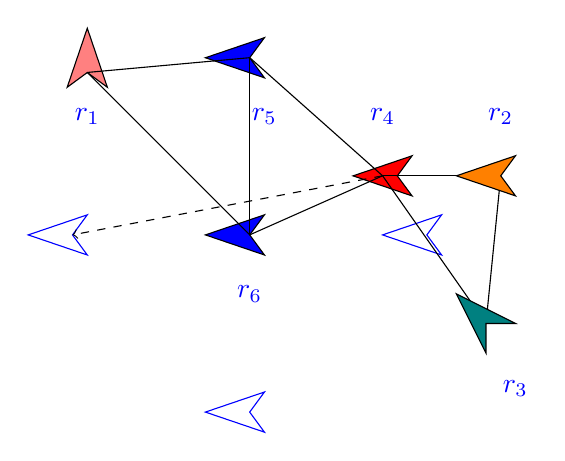
\begin{tikzpicture}[scale=1.5]
    %\useasboundingbox (1,0.5) rectangle (5.5,5);
    % center 2.875 2.75
    \coordinate (S) at (2.875, 2.75);
    \def\shifty{1}
    \def\ddy{2.5}
    \coordinate (A) at (1.5, 4.125);
    \coordinate (B) at (4,4.25-\shifty);
    \draw[fill=blue] (3,2.92) -- (2.5,2.75) -- (3,2.58) -- (2.875,2.75) -- cycle;
    \def\offset{0.5}
    \node[color=blue] at (2.875, 2.75-\offset) {$r_6$};
    % vacancies
    \def\dx{1.5}
    \def\dy{1.5}
    \draw[color=blue] (3+\dx,2.92) -- (2.5+\dx,2.75) -- (3+\dx,2.58) -- (2.875+\dx,2.75) -- cycle;
    \draw[color=blue] (3-\dx,2.92) -- (2.5-\dx,2.75) -- (3-\dx,2.58) -- (2.875-\dx,2.75) -- cycle;
    %%%%%%%
    \draw[fill=blue] (3,2.92+\dy) -- (2.5,2.75+\dy) -- (3,2.58+\dy) -- (2.875,2.75+\dy) -- cycle;
    \node[color=blue] at (3, 3.25+\offset) {$r_5$};
    %%%%%%%%
    \draw[color=blue] (3,2.92-\dy) -- (2.5,2.75-\dy) -- (3,2.58-\dy) -- (2.875,2.75-\dy) -- cycle;
    % another two robots
    \draw[fill=red!50] (1.5,4.5) -- (1.33,4) -- (1.5,4.125) -- (1.67,4) -- cycle; % center .5 4.125
    \node[color=blue] at (1.5, 3.25+\offset) {$r_1$};
    \def\shiftx{1.25}
    \draw[fill=red] (3+\shiftx,3.42) -- (2.5+\shiftx,3.25) -- (3+\shiftx,3.08) -- (2.875+\shiftx,3.25) -- cycle;          
    \node[color=blue] at (4, 4.75-\shifty) {$r_4$};
    \draw[] (S) -- (A);
    \draw[] (S) -- (B);
    \coordinate (V) at (2.875-\dx,2.75);
    \draw[dashed, ->] (B) -- (V);
    % two children of r_i
    \coordinate (C) at  (5, 3.25);
    %\draw[fill=orange] (5,3.5) -- (4.83,3) -- (5, 3.25) -- (5.17,3) -- cycle; % center .\5 3.625
    \node[color=blue] at (5, 3.75) {$r_2$};
    % center or r_c
    \def\xcc{5}
    \def\ycc{3.25}
    \def\hrlen{0.375}
    \def\ylen{0.17}
    \def\xlen{0.125}
    \coordinate (CC) at (\xcc, \ycc);
    % center of r_d
    \def\xdc{4.875}
    \def\ydc{2}
    \def\longlen{0.25}
    \coordinate (DC) at (\xdc, \ydc);
    \draw[] (B) -- (CC);
    \draw[] (B) -- (DC);
    \draw[] (CC) -- (DC);
    \coordinate (CA) at (\xcc-\hrlen, \ycc);
    \coordinate (CB) at (\xcc+\xlen, \ycc+\ylen);
    \coordinate (CD) at (\xcc+\xlen, \ycc-\ylen);
    \draw[fill=orange] (CA) -- (CB) -- (CC) -- (CD) -- cycle;
    \coordinate (D) at (5.375-\offset, 4.5-\ddy);

    \node[color=blue] at (5.125, 3.95-\ddy) {$r_3$};

  
    \coordinate (DA) at (\xdc-\longlen, \ydc+\longlen);
    \coordinate (DB) at (\xdc, \ydc-\longlen);
    \coordinate (DD) at (\xdc+\longlen, \ydc);
    \draw[fill=teal] (DA) -- (DB) -- (DC) -- (DD) -- cycle;
    
    \coordinate (R5) at (2.875, 2.75+\dy);
    \draw[] (S) -- (R5);
    \draw[] (R5) -- (A);
    \draw[] (R5) -- (B);
  \end{tikzpicture}
  \caption{Robot $r_6$ be a stable robot, it has three neighbors
    $r_1, r_5, r_4$ and three vacancies (hollow).  
    Robot $r_4$ is the relocate robot
    and its ultimate destination is the vacancy ahead of
    $r_6$. }
  